% REVISÃO DA LITERATURA--------------------------------------------------------

% \chapter{Revisão da Literatura}
% \label{chap:revisao_da_literatura}

% Para um melhor entendimento do presente trabalho, as Seções \ref{sec:esteganografia} a \ref{sec:stegdeeplearning} apresentam os principais conceitos de esteganografia, esteganálise e redes neurais (com foco em abordagens de aprendizagem profunda). Também serão apresentados os conceitos dos algoritmos de esteganálise e esteganografia relevantes para a avaliação dos resultados.
% avaliação dos resultados - em termos do que?

%------------------------------------------------------------------------

\chapter{Definições}
\label{chap:definicoes}

	Nas próximas seções estão definidos conceitos utilizados neste trabalho, como quadro (\textit{frame}), vídeo e tomada, além da definição de assinatura de vídeo e algumas características consideradas importantes na geração destas. 
    
  	\section{Definição de Vídeo}
    \label{sec:video}
    
    \subsection*{Quadro}
    \label{subsec:quadro}
    Um quadro (ou \textit{frame}) $I$ é uma matriz de altura $h$ e largura $w$. Cada ponto $I[x,y]$ representa uma intensidade de pixel.
    
    , pode ser definido como uma imagem $I$ que possui uma altura e uma largura, cuja intensidade dos \textit{pixels} pode ser representada pela função $f(x,y)$, na qual $x$ representa a posição relativa à largura e $y$ à altura \citeauthorsimoes2004detecccao}. Além disso, um quadro possuí um determinado tempo, que representa o instante em que aparece em um vídeo. Portanto, seguindo a definição de \citeauthorsimoes2004detecccao}, um vídeo é representado por uma sequência de quadros, todos dispostos através da amostra temporal.
    
    
    Um vídeo pode ser segmentado em cenas, que por sua vez possuem diferentes tomadas, compostas por diferentes quadros em sequência, conforme Figura \ref{fig:video}. 
    
    
%     \section{Definição de Tomadas}
%     \label{sec:shot}
 
% 	As tomadas de um vídeo (\textit{shot}), como pode ser observado na Figura \ref{fig:video}, são definidas por um ou mais quadros capturados continuamente, representando uma ação ininterrupta no tempo e no espaço \citeauthordavenport1991cinematic}. Um conjunto de tomadas semelhantes, por sua vez, é intitulado de \textit{cena}. 
    
    \begin{figure}[h]
        \centering
        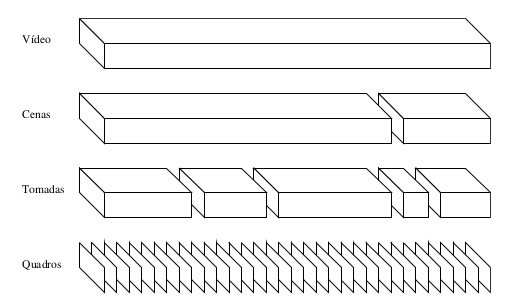
\includegraphics[width=0.96\textwidth]{dados/figuras/video.png}
        \caption{Estrutura de um vídeo. Referência: \citeauthorsantos2004segmentaccao}}
    	\label{fig:video}
    \end{figure}

  	\section{Definição de Assinatura}
    \label{sec:signature}
    
    	Uma assinatura de vídeo é definida como um vetor de características que representa um vídeo e o diferencia de outros \citeauthorlee2008robust}. Outro termo utilizado para fazer essa referência é o de descritor, uma vez que a assinatura irá descrever um determinado vídeo. As características do vídeo podem ser obtidas de diferentes formas, as quais serão apresentadas na seção \ref{sec:desenv}.
        
       Para um algoritmo de geração de assinatura ser considerado eficiente, é importante que três características sejam consideradas: robustez, singularidade e eficiência de busca. De acordo com \citeauthorlee2008robust}, uma assinatura é considerada robusta caso o descritor gerado para um vídeo modificado seja similar ao descritor do vídeo original. A singularidade é a capacidade do algoritmo de gerar assinaturas diferentes para vídeos perceptivelmente diferentes. Por fim, eficiência de busca é a capacidade da assinatura  ser utilizada por uma aplicação para buscas em banco de dados de larga escala. Nesta monografia, são avaliados apenas a robustez e a singularidade das assinaturas.
        
        \subsection{Tipos de descritores de vídeo}
        
        [Procurar um artigo que defina os descritores +- dentro do que implementamos, e escrever um parágrafo explicando que vamos seguir as definições daquele artigo, já que não existe uma convenção sobre o que são descritores globais e locais.]


	Os descritores de vídeo podem ser classificados em dois tipos: globais e locais. De acordo com \citeauthorde2012combinaccao}, o primeiro busca informações pertinentes ao quadro como um todo, como por exemplo um histograma de cores de toda a imagem. Outros exemplos de características globais são texturas, bordas e formas  \citeauthorlaw2007video}.
       
    Características locais, por sua vez, procuram por pontos de interesse ou regiões específicas no quadro, utilizando, por exemplo, algoritmos como SIFT, SURF ou LBP (\textit{Local Binary Pattern}), entre outros.      
    
    COLOCAR IMAGEM DO SIFT OU SEI LA

\chapter{Estado da Arte}
\label{chap:estadodaarte}

  	% Problemas
  	  % cbvr
      % cbcd
      % cbir
     \section{Detecção de Cópias Baseada em Conteúdo} 
	Segundo \citeauthorjiang2011pku}, o método de detecção de cópias baseada em conteúdo, do inglês \textit{Content Based Copy Detection} (CBCD), tem se tornado uma alternativa à marca d'água, conforme ilustra a Figura \ref{fig:marcadagua}, para identificar e proteger vídeos e seus direitos autorais através da criação de uma assinatura digital para o conteúdo. Apesar de o método CBCD vir sendo largamente utilizado em diversas aplicações, a detecção de cópias é um grande desafio e o trabalho de \citeauthorjiang2011pku} expõe determinadas limitações do método.
    
    O conteúdo a ser procurado pode sofrer uma intensa redução em sua qualidade entre o vídeo original e a cópia, podendo até mesmo sofrer alterações, como por exemplo, distorções e transformações. É uma tarefa difícil buscar cópias através de mecanismos baseados em pesquisa por quadros sem uma ferramenta que consiga unir corretamente a duração de cada trecho a ser pesquisado com o vídeo original. Por último, é necessária uma representação compacta e eficiente das assinaturas para que se construa uma ferramenta de busca e detecção de cópias para grandes sistemas.
    
    	\begin{figure}[h]
        \centering
        
\includegraphics[width=0.4\textwidth]{dados/figuras/marca_dagua.png}
        \caption{Exemplo de marca d'água em uma imagem.}
    	\label{fig:marcadagua}
    \end{figure}

\section{Recuperação de Vídeo Baseada em Conteúdo}
De acordo com \citeauthorlaw2007video}, recuperação de vídeo baseado em conteúdo, do inglês \textit{Content Based Video Retrieval} (CBVR) é o procedimento para gerar, pesquisar e analisar assinaturas digitais. Essa área de estudo produz os algoritmos que geram os identificadores digitais, estuda a similaridade entre assinaturas e também busca trechos em vídeos. Ainda segundo \citeauthorlaw2007video}, CBVR tem foco em procurar e encontrar vídeos em uma mesma categoria, como por exemplo, jogos de futebol ou vídeos sobre balões.

\section{Recuperação de Imagens Baseada em Conteúdo}
Conforme \citeauthorgudivada1995content}, recuperação de imagens baseada em conteúdo, em inglês \textit{Content Based Image Retrieval} (CBIR), é um sistema que auxilia na recuperação e extração de imagens de acordo com o conteúdo da imagem. Para representar uma imagem, o sistema CBIR se baseia em elementos visuais como cores, texturas e formas \citeauthorvikhar2016improved}. Há diversas aplicações que se beneficiam desta tecnologia, como: previsão do tempo, serviços de informações geográficas, design de interiores, galerias de arte, etc \citeauthorgudivada1995content}.

\chapter{Trabalhos relacionados}
\label{chap:relacionados}

  % Artigo 9 - 372: Ele fala de técnicas na história - comparar cenas (final/inicio): comparar descritores; - transformação pós-produção: utilização de pontos de interesse;

Existem diversos trabalhos correlatos que discutem assuntos como assinatura digital de vídeos, formas de obter as descrições, analisar e comparar assinaturas, métodos para realizar buscas em vídeos, descritores globais e locais, etc. 

Em 1999, quando a visualização de vídeos na internet ainda estava em sua infância, \citeauthorindyk1999finding} já buscava métodos para encontrar vídeos pirateados na web. Este propôs um algoritmo para geração de assinatura temporal baseada nos limites das cenas de um vídeo. Embora seja boa para encontrar filmes inteiros, esta técnica não é apropriada para vídeos curtos, que dominam as redes sociais de vídeos (aproximadamente 4 minutos) \citeauthorcomscoreinc}.

Desde então, várias técnicas têm sido usadas para a geração de assinaturas. \citeauthorcoskun2006spatio} propôs o conceito de funções de \textit{hash} como uma ferramenta para identificação de vídeo, criando uma algoritmo espaço-temporal baseado no diferencial da luminância entre regiões de quadros. Outras abordagens incluem o uso de descritores globais que utilizam a distribuição da intensidade de movimento e cor \citeauthorhampapur2001comparison}, além de medidas ordinais \citeauthorhua2004robust}, que se provaram robustas para variadas resoluções, mudanças de iluminação e formatos de vídeos.	   	

Abordagens que utilizam características locais também foram extensamente pesquisadas, como em \citeauthorjoly2007content}, cujo algoritmo apresentado busca ser eficiente para buscas em grandes bases de dados, tanto em velocidade quanto a qualidade. Há também a  pesquisa de \citeauthorlaw2006robust}, que usa o algoritmo de Harris para encontrar pontos de interesse no vídeo e criar uma assinatura compacta.

\citeauthorde2012combinaccao} fez um estudo comparativo entre descritores globais e locais e mostrou como unir os dois tipos de descritores através de algoritmos genéticos. \citeauthorde2012combinaccao} também fez vários experimentos mostrando que a combinação de descritores globais e locais são complementares e se usados em conjunto, produzem resultados superiores quando comparados com o uso individual de cada tipo de descritor.

\citeauthorhu2011survey} discorre sobre a indexação e recuperação de conteúdo em vídeos. O trabalho apresenta métodos para analisar a estrutura de vídeos, segmentação de cenas, extração de quadros-chave, características de movimento, mineração de informações em vídeos, mensuramento de similaridade e relevância entre assinaturas digitais, pesquisa de conteúdo em vídeos entre outros.

% Na área de descritores globais e locais, \citeauthorchen2008video} apresenta uma abordagem temporal, ou seja, não se limitar a dizer se uma determinada sequência de \textit{frames} pode estar presente em um vídeo, mas se estiver, em qual parte do vídeo esse trecho se encontra.
